\subsection{SimpleCNN}\label{resultsSimpleCNN}

After establishing the basic architecture of our SimpleCNN (as described in Section~\ref{simplecnn}), our next goal was to effectively classify the first digits of the dataset. This required the selection of initial hyperparameters to begin the training and evaluation process. Without prior benchmarks, we initially decided on a batch size of 8, set the number of epochs to 5 and a learning rate of 0.1. However, this initial configuration led to less satisfactory results, which made us to revise our hyperparameters to improve performance.

The training process was completed relatively quickly so that we could implement a function to test the hyperparameters. This required us to set default values for each training and evaluation session, with certain values being adjusted at each iteration. For example, we set the batch size to 32, the learning rate to 0.001 and the epochs to 15. In subsequent runs, we changed one hyperparameter at a time, while keeping the others constant. This means that we ran training sessions with learning rates of 0.001, 0.01 and 0.1, respectively, while keeping the default values for batch size and epochs. Similarly, we experimented with different batch sizes and varied the number of epochs. This systematic approach allowed us to evaluate the effects of each hyperparameter. The following code snippedt provides a brief summary of the hyperparameters that were explored during this process:

\begin{minted}[mathescape, linenos, fontsize=\small]
{python}
    ...
    # Hyperparameters
    num_classes = 10
    default_lr = 0.001
    default_bs = 32
    default_epoch = 15
    learning_rates = [default_lr, 0.01, 0.1]
    batch_sizes = [16, default_bs, 64]
    num_epochs = [5, 10, default_epoch, 20]
    ...
\end{minted}

After analyzing the experimental data (see Appendix, Table~\ref{table:lr_bs_ep}), we discovered the most effective hyperparameters for our SimpleCNN model, and interestingly, we found that the default values were already optimal. We obtained these results with the original SimpleCNN architecture. Subsequently, we applied these hyperparameters to train an updated version of the SimpleCNN\@. To assess the impact of the changes, we compared the performance of the original and updated architectures. The comparative analysis is shown in Figure~\ref{fig:SimpleCNN_old_new}.

\begin{figure} [ht]
    \centering
    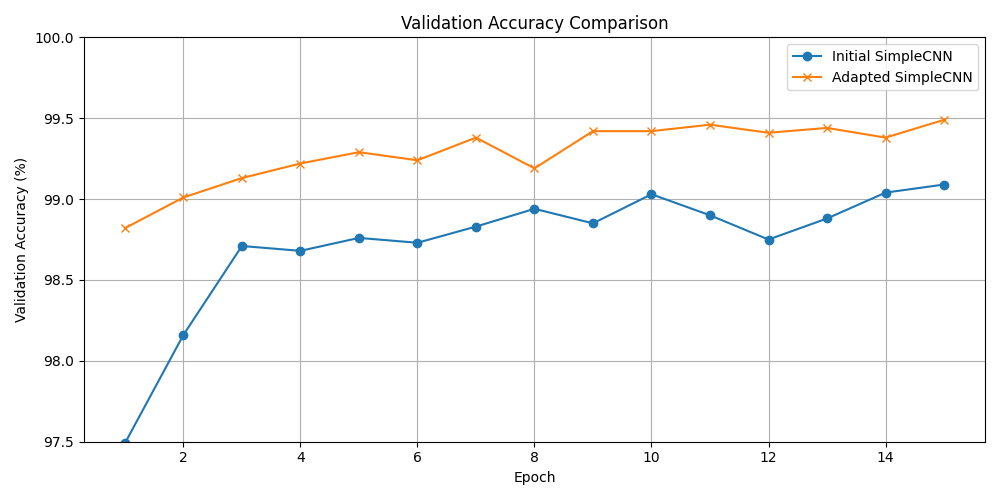
\includegraphics[width=.9\textwidth]{figures/simpleCNN_old_vs_new.png}
    \caption{Comparison of validation accuracy across epochs between the initial and the adapted SimpleCNN model, highlighting the overall improved performance of the adapted model.}\label{fig:SimpleCNN_old_new}
\end{figure}

For the second challenge, which focused on the PathMNIST dataset, our approach exclusively used the customized version of our SimpleCNN architecture due to its better performance. To combat overfitting, we introduced an early stopping mechanism. The core of this experiment was to assess the impact of incorporating batch normalization and dropout techniques. We conducted three separate trials: one with both batch normalization and dropout, one with only dropout, and another with only batch normalization. The outcomes of these trials can be seen in Figure~\ref{fig:pathMNIST_variations}.

\begin{figure} [ht]
  \centering
  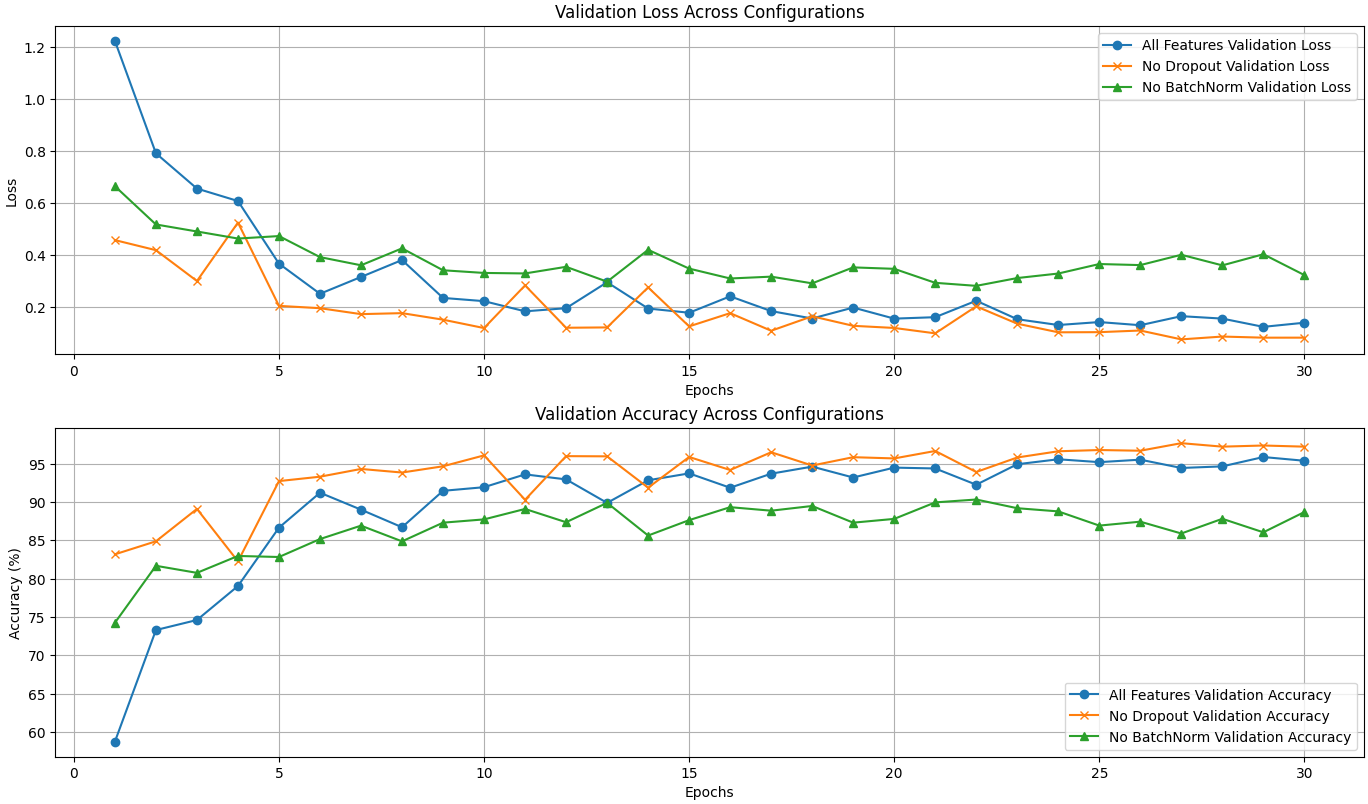
\includegraphics[width=1\textwidth]{figures/simpleCNN_PathMNIST_variations.png}
  \caption{Performance comparison of SimpleCNN variations on the PathMNIST dataset over 30 epochs.}\label{fig:pathMNIST_variations}
\end{figure}